\chapter{Shai Lèger Hernández}
	
	\begin{figure}[h]
		\centering
		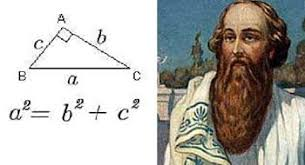
\includegraphics[scale=1]{./IMG/5.png}     
		\caption{Imagen de prueba}
		\label{fig:prueba}
	\end{figure}

\section{Sobre mi}

     - Tengo 18 años, tengo nacionalidad Canadiense, mi apellido es francés, mi nombre es hebreo.
     
\section{Hobbies}

	\begin{itemize}
		\item Programación
		\item Piano
	\end{itemize}
	
%referencias
%El \textbf{Teorema}-\ref{fig:prueba}

\newpage
\chapter{Cosas de matemáticas}

\section{Formulas}

	\begin{itemize}
		\begin{huge}
			\item {$c^{2} = a^{2} + b^{2}$}\\
			\item {$x =\frac{-b \pm \sqrt{b^{2} - 4ac}}{2a}$}\\
		\end{huge}
	\end{itemize}


\section{Tabla de ley de los simbolos}

	\begin{table}[h]
		\centering
		
		\label{tab:leyes_signos}
		\begin{tabular}{ | c | c | c | }
			
			\hline
			Operando & Operando & Resultado\\
			\hline
			$+$ & $+$ & $+$\\
			$+$ & $-$ & $-$\\
			$-$ & $+$ & $-$\\
			$-$ & $-$ & $+$\\
			\hline
			
		\end{tabular}
		\caption{Tabla de signos}
	\end{table}
	
	\centering\emph{Plantilla para hacer una \emph{Tabla}~\ref{tab:leyes_signos} en \LaTeX}
		
